\documentclass{article}
\author{Victor Mittermair, 11809916}
\usepackage{hyperref}
\usepackage{fancyhdr}
\usepackage{tikz} 
\usepackage{amsthm}
\usepackage{verbatim}
\usepackage{subfigure}
\usepackage{amssymb}
\usepackage{mathtools}
\usepackage{amsmath}
\usepackage{soul}
\usepackage{algorithm}
\usepackage{algpseudocode}
\usepackage{algorithmicx}

\newtheorem*{theorem}{Theorem}
\newtheorem*{lemma}{Lemma}
\theoremstyle{definition}
\newtheorem*{definition}{Definition}
\theoremstyle{remark}
\newtheorem*{remark}{Remark}
\newtheorem*{note}{Note}
\newtheorem*{statement}{Statement}
\newtheorem*{example}{Example}

%\lhead{\includegraphics[width=0.2\textwidth]{nyush-logo.pdf}}
\fancypagestyle{firstpage}{%
  \lhead{TU Vienna}
  \rhead{
  Discrete Math for Informatics WS 2022}
}

%%%% PROJECT TITLE
\title{Discrete Math for Informatics\\
        \Large \emph{3rd Lecture}}


\date{\today} %NO DATE



\begin{document}
\maketitle
\thispagestyle{firstpage}


\begin{comment}
\section*{Graph}
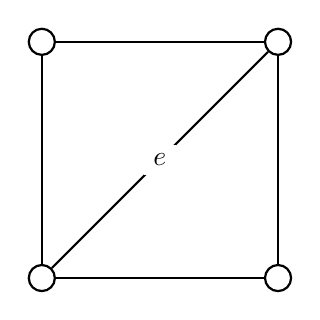
\begin{tikzpicture}[node distance={30mm}, thick, main/.style = {draw, circle}]
    \centering
    \node[main] (1)              {}; 
    \node[main] (2) [right of=1] {};
    \node[main] (3) [below of=1] {}; 
    \node[main] (4) [right of=3] {};
    \draw (1) -- (2) ; 
    \draw (1) -- (3); 
    \draw (2) -- (4); 
    \draw (3) -- (4);
    \draw (3) -- (2) node [midway, fill=white] {$e$}; 
\end{tikzpicture}


\begin{equation}
    \sum_{n = 1}^{\infty} 2n \approx \int_{a}^{b} 2x \,dx 
\end{equation}

\begin{proof}
    Lorem ipsum
\end{proof}

\begin{remark}
    Lorem ipsum

\end{remark}

\begin{definition}[Walk]
    Lorem ipsum
\end{definition}

\begin{theorem}
    Lorem ipsum.
\end{theorem}

\begin{lemma}[Handshake-lemma]
    Lorem ipsum.
\end{lemma}
\end{comment}

\subsection*{Kruskal Spanning tree of minimal weight}
Assume graph G is connected:
\begin{algorithm}
    
    \begin{algorithmic}
    \Require Sorted edges by weight: $w(e_1) \leq ... \leq w(e_m)$.
    \State $T_1 \gets \emptyset$
    \For{$i$ in $1...m$}
        \If{$E(T_i) \cup e_i$ is acyclic}
            \State $E(T_{i+1}) \gets E(T_i) \sqcup e_i $
        \Else
            \State $E(T_{i+1}) \gets E(T_i) $
        \EndIf
        \If{$|E(T_{i+1}|+1=n-1$}
            \State \textbf{return} $E(T) \gets E(T_{i+1}$)
        \EndIf
    \EndFor
    \end{algorithmic}
\end{algorithm}
\begin{remark}
    Kurskal is a so greedy algorithm: add best looking edge
\end{remark}
\begin{theorem}
    Kruskal yields a spanning tree of minimal weight
\end{theorem}
\begin{proof}
    $ $\\
    \begin{itemize}
        \item $T$ is acyclic by construction.
        \item Suppose the algorithm reaches the return statement and $T_{m+1}$ is not connectced with components $A$ and $B$. There has to be an edge $e_l$ which connects the two components $A$ and $B$. Kruskal would habe added $e_l$ becuase $T_l \subseteq T_{m+1}$ is acyclic.
        \item T is of minimal weight: see proof in matroid setting
    \end{itemize} 
\end{proof}
\subsection*{Metroids}
\textbf{Metroids} provide a framework for greedy algorithms.
\begin{definition}
    let $E$ be a set, $I$ a set of subsets of $E$. the set of independant sets\\
    $M1: \emptyset \in I$\\
    $M2: B \in I, A \subseteq B \rightarrow A \in I$\\
    $M3: A,B \in I, |B| = |A| + 1 \Rightarrow \exists e \in B \backslash A: A \cup {e} \in I$\\ "exchange axiom"
    Then $(E,I)$ is a \textbf{matroid}.
\end{definition}
\begin{theorem}
    $G$ a graph, $I:=\{F \subset E(G) | F \text{ acyclic} \} \Rightarrow (E,I)$ is a matroid
\end{theorem}
\begin{proof}
    M1: $\emptyset$ is a forest, M2: $B$ is a forest $A \subseteq B \Rightarrow A$ is a forest
    M3: $A,B$ edge sets of spanning forests, $|B|=|A| + 1$, find edge $e \in B \backslash A$ such that $A \cup e$ is a forest.\\
    Suppose $A$ has connecdted components $T_1 ... T_c$
    Show $\exists e$ in $B\backslash A$ that is not in any of these components.
    count edges:
    %formula 1
    %formula 2
    $B$ has more than $|A|$ edges, so there is an edge not in any $B$ restricted by $V(T_i)$
\end{proof}
\begin{algorithm}
    Greedy: $(E,I)$ matroid, $w: E \rightarrow \mathbb{R}$ 
    \begin{algorithmic}
    \Require Sorted E by weight: $w(e_1) \leq ... \leq w(e_m)$.
    \State $T_1 \gets \emptyset$
    \For{$i$ in $1...m$}
        \If{$E(T_i) \cup e_i$ $\in I$}
            \State $E(T_{i+1}) \gets E(T_i) \sqcup e_i $
        \Else
            \State $E(T_{i+1}) \gets E(T_i) $
        \EndIf
    
       
    \EndFor
    \State \textbf{return} $E(T) \gets E(T_{m+1}$)
    \end{algorithmic}
\end{algorithm}
\begin{definition}
    A \textbf{basis} of a matroid is a (inclusionwise) maximal independent set.
\end{definition}
\begin{theorem}
    Greedy returns a basis of minimal weight, that is $\sum_{e\in T} w(e)$ is minimal among all bases.
\end{theorem}
\begin{proof}
    $T$ is a maximal independent set as in Kruskal.\\
    $\sum_{e \in T}w(e)$ is minimal: let $T= \{t_1,...,t_s\} w(t_1) \leq ... \leq w(t_s)$\\
    suppose that $B=\{b_1,...,b_r\}$ with $w(b_1) \leq .. \leq w(b_r)$ is a basis with $\sum_{b \in B} w(b) < \sum_{e \in T}w(e)$\\
    let $i:= min\{j | w(b_j) < w(t_j)\}$ ie, $w(b_j) \geq w(t_j)$ for $j < i$ and $w(b_j) < w(t_i)$
    let $T_{i-1} = \{t_1,..,t_{i-1}\} B_i = \{b_1, ..., b_i\}$\\
    apply $M3$\\
    $\Rightarrow \exists b_j \in B_i \backslash T_{i-1}: T_{i-1} \cup b_j \in I$\\
    $w(b_j) \leq w(b_i) < w(t_i)$ so greedy should have chosen $b_j$ instead of $t_i$\\
    $j$ with $w(b_j) < w(t_j)$ exists becuase all bases have the same cordinality.
\end{proof}
\begin{theorem}
    suppose that $(E,I)$ satisfies $M1$ and $M2$, and that for any weight function $w: E \rightarrow \mathbb{R}$ the greedy algorithm produces a maximal independent set $A \in I$ such that $\sum_{e\in A}w(e)$ is minimal among all maximal sets in $I$. Then $(E,I)$ satisfies $M3$, ie is a matroid.
\end{theorem}
\begin{proof}
    $ $\\
    \begin{itemize}
        \item all maximal sets in $I$ have the same cardinality. Suppose $A,B \in I$ maximal, $|A|<|B|$
        %formula 3
        (we will determine $\epsilon >0$ in a suitable way).\\ for any $\epsilon > 0$ greedy returns B. $w(B) = |B|\geq |A| + 1$ \\
        $w(A) = |A \cap B| + (1+\epsilon)|A\backslash B|=|A|+\epsilon|A\backslash B| \Rightarrow$ choose $\epsilon < \frac{1}{|A\backslash B|}$ ($A\backslash B \neq \emptyset )$
        \item $(E,I)$ satisfies $M3$, let $A,b \in I, |B|=|A|+1 $ \\%formula 4
        greedy chooses all of $A$ first: since $|A|<|B|$ we have that $A$ is not maximal\\ suppose $\nexists e \in B \backslash A | A \cup e \in I$\\
        $\Rightarrow$ greedy chooses $r-|A|$ elements of weight $x$, where $r$ is the size of any basis. call this set $A^\prime$, also $\exists$ basis $B^\prime=B\cup \{e_1,...e_{r-|B|}\}$ \\
        $w(A^\prime) = w(A) + x(r-|A|) = x(r-|A|)$\\
        $w(B^\prime)\leq |B\backslash A| + x(r-|B|)= |B\backslash A| + x(r-|A|-1) \leq w(A^\prime) + |B\backslash A|-x$\\
        $\Rightarrow$ choose $x > |B\backslash A|$, then $w(B^\prime) < w(A^\prime)$ but greedy returned $A^\prime$
    \end{itemize}
\end{proof}

\begin{algorithm}
    Prims algorithm: let G connected, r any vertex
    \begin{algorithmic}
    \Require Sorted E by weight: $w(e_1) \leq ... \leq w(e_m)$.
    \State $Q \gets V(G)\backslash r$
    \State $T \gets \emptyset$
    \State $V_T \gets \{r\}$
    \While{$Q \neq \emptyset$}
        \State $u \gets$ a vertex in $Q$ connected to $T$ with an edge of minimal weight
        \State $Q \gets Q \backslash u$
        \State $T \gets T \cup e$
        \State $V_T \gets V_T \cup u$
    \EndWhile
    \end{algorithmic}
\end{algorithm}
Prim is a greedy algorithm, but there is no matroid underlying
\end{document}